\section{\textit{Markov Chain Monte Carlo} - MCMC}

\subsection{Leituras Recomendadas}
\begin{frame}{\textit{Markov Chain Monte Carlo} - MCMC - Leituras Recomendadas}
    \begin{vfilleditems}
        \item \textcite{gelman2013bayesian}
        \begin{vfilleditems}
            \item Capítulo 10: Introduction to Bayesian computation
            \item Capítulo 11: Basics of Markov chain simulation
            \item Capítulo 12: Computationally efficient Markov chain simulation
        \end{vfilleditems}
        \item \textcite{mcelreath2020statistical} - Capítulo 9: Markov Chain Monte Carlo
        \item \textcite{neal2011mcmc}
        \item \textcite{betancourtConceptualIntroductionHamiltonian2017}
        \item \textcite{gelman2020regression} - Capítulo 22, Seção 22.8: Computational efficiency
        \item \textcite{storopoli2021estatisticabayesianaR} - Markov Chain Monte Carlo
        \item \textcite{chibUnderstandingMetropolisHastingsAlgorithm1995}
        \item \textcite{casellaExplainingGibbsSampler1992}
    \end{vfilleditems}
\end{frame}

\begin{frame}{Métodos de Monte Carlo}
  \begin{columns}
    \begin{column}{0.8\textwidth}
      \begin{vfilleditems}
        \item \href{http://mc-stan.org/}{\texttt{Stan}} é uma homenagem ao matemático
        Stanislaw Ulam, que participou do projeto Manhattan e ao tentar calcular o
        processo de difusão de neutrons para a bomba de hidrogênio acabou criando uma
        classe de métodos chamada \textbf{Monte Carlo} \parencite{eckhardtStanUlamJohn1987}.
        \item Métodos de Monte Carlo possuem como conceito subjacente o uso a aleatoriedade
        para resolver problemas que podem ser determinísticos em princípio.
        Eles são freqüentemente usados em problemas físicos e matemáticos e
        são mais úteis quando é difícil ou impossível usar outras abordagens.
      \end{vfilleditems}
    \end{column}
    \begin{column}{0.2\textwidth}
      \centering
      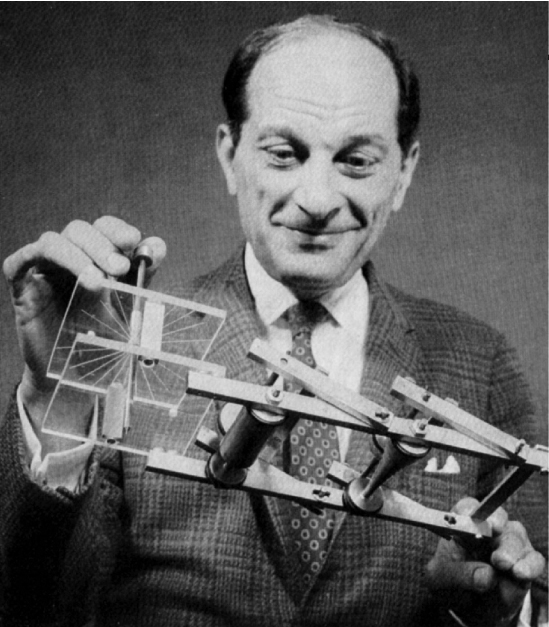
\includegraphics[width=0.9\columnwidth]{stanislaw.jpg}
    \end{column}
  \end{columns}
\end{frame}

\begin{frame}{História dos Métodos de Monte Carlo\footnote{para quem se interessou, a história se encontra em \textcite{eckhardtStanUlamJohn1987}}}
  \begin{columns}
    \begin{column}{0.8\textwidth}
      \begin{vfilleditems}
        \item A ideia do método veio enquanto jogava paciência durante sua
        recuperação de uma cirurgia, Ulam pensou em jogar centenas de jogos para
        estimar estatisticamente a probabilidade de um resultado bem-sucedido
        \item Ulam descreveu a ideia para John von Neumann em 1946
        \item \small Por ser secreto, o trabalho de von Neumann e Ulam exigia um codinome.
        Um colega de von Neumann e Ulam, Nicholas Metropolis, sugeriu usar o nome Monte Carlo,
        que se refere ao Casino Monte Carlo em Mônaco, onde o tio de Ulam (Michał Ulam)
        pedia dinheiro emprestado a parentes para jogar.
      \end{vfilleditems}
    \end{column}
    \begin{column}{0.2\textwidth}
      \centering
      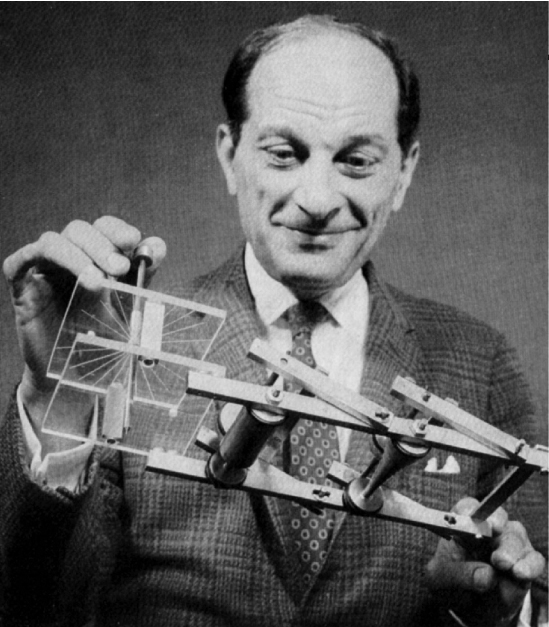
\includegraphics[width=0.9\columnwidth]{stanislaw.jpg}
    \end{column}
  \end{columns}
\end{frame}

\subsection{Por quê Precisamos de MCMC?}
\begin{frame}{Por quê Precisamos de MCMC?}
  A principal barreira computacional para estatística Bayesiana é o denominador
  $P(\text{data})$ da fórmula de Bayes:

  $$P(\theta \mid \text{data})=\frac{P(\theta) \cdot P(\text{data} \mid \theta)}{P(\text{data})}$$

  Em casos discretos podemos fazer o denominador virar a soma de todos os parâmetros
  usando a \textbf{regra da cadeia de probabilidade} (\textit{chain rule}):

  $$P(A,B \mid C)=P(A \mid B,C) \times P(B \mid C)$$

  Isto também é chamado de \textbf{marginalização}:

  $$P(\text{data})=\sum_{\theta} P(\text{data} \mid \theta) \times P(\theta)$$
\end{frame}

\begin{frame}{Por quê Precisamos de MCMC?}
  Porém no caso de valores contínuos o denominador $P(\text{data})$ vira uma integral
  bem grande e complicada de calcular:

  $$P(\text{data})=\int_{\theta} P(\text{data} \mid \theta) \times P(\theta)d \theta$$

  Em muitos casos essa integral vira \textit{intratável} (incalculável) e
  portanto devemos achar outras maneiras de calcular a probabilidade posterior
  $P(\theta \mid \text{data})$ de Bayes sem usar o denominador $P(\text{data})$.
  \vfill
  \Large \textbf{É aqui que entra Métodos de Monte Carlo!}
\end{frame}

\begin{frame}{Para quê serve o denominador $P(\text{data})$}
  Para normalizar a posterior com o intuito de torná-la uma distribuição
  probabilística válida. Isto quer dizer que a soma de todas as probabilidades
  dos eventos possíveis da distribuição devem ser iguais a $1$:
  \begin{vfilleditems}
    \item no caso de distribuição probabilística \textbf{discreta}:
    $$\sum_{\theta} P(\theta \mid \text{data}) = 1$$
    \item no caso de distribuição probabilística \textbf{contínua}:
    $$\int_{\theta} P(\theta \mid \text{data})d \theta = 1$$
  \end{vfilleditems}
\end{frame}

\begin{frame}{Se removermos o denominador de Bayes o que temos?}
  Ao removermos o denominador $(\text{data})$ temos que a posterior
  $P(\theta \mid \text{data})$ é \textbf{proporcional} à \textit{priori}
  multiplicada pela verossimilhança $P(\theta) \cdot P(\text{data} \mid \theta)$:

  $$P(\theta \mid \text{data}) \propto P(\theta) \cdot P(\text{data} \mid \theta)$$

\end{frame}

\subsubsection{Correntes Markov}
\begin{frame}{Método de Montecarlo com Correntes Markov -- (MCMC)}
  Aí que entra \textbf{Método Montecarlo com Correntes Markov}\footnote{do inglês
  \textit{Markov Chain Monte Carlo} (MCMC)}.
  \vfill
  MCMC é uma classe ampla de ferramentas computacionais para aproximação
  de integrais e geração de amostras de uma probabilidade posterior
  \parencite{brooksHandbookMarkovChain2011}.
  \vfill
  MCMC é usada quando não é possível coletar amostras de $\boldsymbol{\theta}$
  direto da distribuição probabilística posterior
  $P(\boldsymbol{\theta} \mid \text{data})$.
  Ao invés disso, nos coletamos amostras de maneira iterativa que a cada passo do
  processo nós esperamos que a distribuição da qual amostramos
  $P^*(\boldsymbol{\theta}^{(*)} \mid \text{data})$
  se torna cada vez mais similar à posterior $P(\boldsymbol{\theta} \mid \text{data})$.
  \vfill
  Tudo isso é para \textbf{eliminar o cálculo} (muitas vezes impossível) do \textbf{denominador} $P(\text{data})$.
\end{frame}

\begin{frame}{Correntes Markov}
  \begin{columns}
    \begin{column}{0.8\textwidth}
      \begin{vfilleditems}
        \item A ideia é \textbf{definir uma corrente Markov ergódica}
        (quer dizer que há uma distribuição estacionária única)
        dos quais o conjunto de estados possíveis é o espaço amostral e a
        distribuição estacionária é a distribuição a ser \textit{aproximada} (ou \textit{amostrada}).
        \item Seja $X_0, X_1, \dots, X_n$ uma simulação da corrente.
        A corrente Markov \textbf{converge à distribuição estacionária de qualquer
        estado inicial} $X_0$ após um \textbf{número suficiente grande de iterações} $r$,
        a distribuição do estado $X_r$ estará similar à distribuição estacionária,
        então podemos usá-la com amostra.
      \end{vfilleditems}
    \end{column}
    \begin{column}{0.2\textwidth}
      \centering
      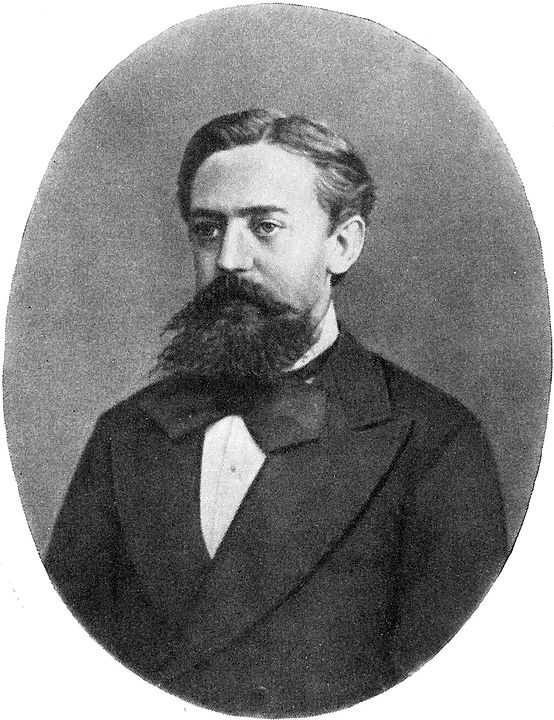
\includegraphics[width=0.9\columnwidth]{andrei_markov.jpg}
    \end{column}
  \end{columns}
\end{frame}

\begin{frame}{Correntes Markov}
  \begin{columns}
    \begin{column}{0.8\textwidth}
      \begin{vfilleditems}
        \item As correntes Markov possuem uma propriedade que a distribuição probabilística
        do próximo estado depende \textbf{apenas do estado atual e não na sequência
        de eventos que precederam}:
        $P(X_{n+1}=x \mid X_{0},X_{1},X_{2},\ldots ,X_{n}) = P(X_{n+1}=x \mid X_{n})$.
        Essa propriedade é chamada de \textbf{Markoviana}.
        \item Similarmente, repetindo esse argumento com $X_r$ como o ponto inicial,
        podemos usar $X_{2r}$ como amostra, e assim por diante.
        Podemos então usar a sequência de estados $X_r, X_{2r}, X_{3r}, \dots$
        como quase \textbf{amostras independentes} da distribuição estacionária da
        corrente Markov.
      \end{vfilleditems}
    \end{column}
    \begin{column}{0.2\textwidth}
      \centering
      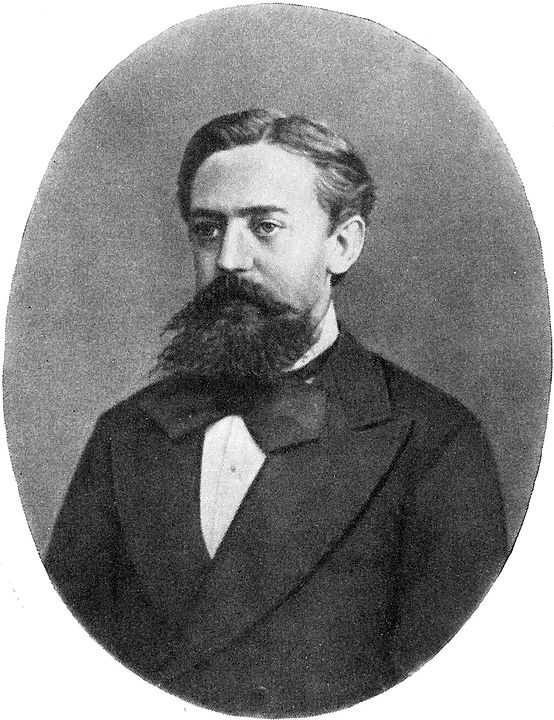
\includegraphics[width=0.9\columnwidth]{andrei_markov.jpg}
    \end{column}
  \end{columns}
\end{frame}

% Idea taken from http://steventhornton.ca/blog/markov-chains-in-latex.html
\begin{frame}{Exemplo de Corrente Markov}
  \centering
  \begin{tikzpicture}
    % Add the states
    \node[state,
    text=yellow,
    minimum size=2cm,
    thick
    ]
    (s) {Sol};
    \node[state,
    right=3cm of s,
    text=blue!30!white,
    minimum size=2cm,
    thick
    ]
    (r) {Chuva};

% Connect the states with arrows
\draw[every loop,
    auto=right,
    line width=1mm,
    >=latex]
  (s) edge[bend right, auto=left]  node {0.6} (r)
  (r) edge[bend right, auto=right] node {0.7} (s)
  (s) edge[loop above]             node {0.4} (s)
  (r) edge[loop above]             node {0.3} (r);
\end{tikzpicture}
\end{frame}

\begin{frame}{Correntes Markov}
  A eficácia dessa abordagem depende em:

  \begin{vfilleditems}
    \item \textbf{o quão grande $r$ deve ser} para garantir uma \textbf{amostra adequadamente boa}
    \item \textbf{poder computacional} requerido para cada iteração da corrente Markov.
  \end{vfilleditems}

  \vfill
  \footnotesize
  Além disso, é costumeiro descartarmos as primeiras iterações do algoritmo pois
  elas costumam não ser representativas da distribuição a ser aproximada.
  Nas iterações iniciais de algoritmos MCMC geralmente a corrente Markov
  está em um processo de aquecimento\footnote{Algumas referências chamam esse processo de \textit{burnin}}
  (\textit{warm-up}) e seu estado está bem distante do ideal para começarmos uma amostragem
  fidedigna.
  \vfill
  Geralmente, recomenda-se que se descarte metade das iterações \parencite{gelmanBasicsMarkovChain2013}.
\end{frame}

\subsection{Algoritmos de MCMC}
\begin{frame}{Algoritmos de MCMC}
  Temos \textbf{MUITOS} algoritmos de MCMC\footnote{Veja a \href{https://en.wikipedia.org/wiki/Markov_chain_Monte_Carlo}{página da Wikipedia para uma listagem completa}}
  Mas aqui vamos cobrir duas classes de algoritmos MCMC:
  \begin{vfilleditems}
    \item Metropolis-Hastings \parencite{metropolisEquationStateCalculations1953, hastingsMonteCarloSampling1970}

    \item Hamiltonian Monte Carlo\footnote{às vezes chamado de \textit{Hybrid Monte Carlo}, especialmente na literatura de Física} \parencite{neal2011mcmc, betancourtConceptualIntroductionHamiltonian2017}
  \end{vfilleditems}
\end{frame}

\begin{frame}{Classe de Algoritmos MCMC -- Metropolis-Hastings}
  Os primeiros algoritmos de MCMC. Usam uma regra de aceitação/rejeição das
  propostas. Caracterizados por propostas oriundas de um passeio aleatório\footnote{\textit{random walk}}
  no espaço amostral. O algoritmo de \textbf{Gibbs} pode ser visto como um
  \textbf{caso especial} do algoritmo de MH porque
  todas as propostas são aceitas \parencite{gelmanIterativeNonIterativeSimulation1992}
  \vfill
  Assintoticamente, possuem uma taxa de aceitação de 23.4\% e o custo de cada iteração é
  $\mathcal{O}(d)$, na qual $d$ é a dimensão do espaço amostral \parencite{beskosOptimalTuningHybrid2013}.
\end{frame}

\begin{frame}{Classe de Algortimos MCMC -- Hamiltonian Monte Carlo}
  Os algoritmos MCMC mais eficientes na atualidade. Tenta evitar o comportamento
  de passeio aleatório introduzindo um vetor de momento auxiliar e
  implementando dinâmicas Hamiltonianas. As propostas são "guiadas"~
  para regiões de maior densidade do espaço amostral. Isso faz com que HMC seja
  \textbf{ordens de magnitude mais eficiente que MH e Gibbs}.
  \vfill
  Assintoticamente, possuem uma taxa de aceitação de 65.1\% e o custo de cada iteração é
  $\mathcal{O}(d^{\frac{1}{4}})$, na qual $d$ é a dimensão do espaço amostral \parencite{beskosOptimalTuningHybrid2013}.
\end{frame}

\subsubsection{Metropolis}
\begin{frame}{Algoritmo de Metropolis}
  \begin{columns}
    \begin{column}{0.8\textwidth}
      O primeiro algoritmo MCMC amplamente utilizado para gerar amostras de
      correntes Markov foi originário na física na década de 1950 e chama-se Metropolis
      \parencite{metropolisEquationStateCalculations1953} em homenagem ao primeiro
      autor \href{https://en.wikipedia.org/wiki/Nicholas_Metropolis}{Nicholas Metropolis}.
      \vfill
      Em síntese, o algoritmo de Metropolis é uma adaptação de um passeio aleatório
      com uma regra de aceitação/rejeição para convergir à distribuição-alvo.
      \vfill
      O algorimo de Metropolis usa uma \textbf{distribuição de propostas}
      $J_t(\boldsymbol{\theta}^{(*)})$
      para definir próximos valores da distribuição
      $P^*(\boldsymbol{\theta}^{(*)} \mid \text{data})$.
      Essa distribuição deve ser simétrica:
      $$
      J_t (\boldsymbol{\theta}^{(*)} \mid \boldsymbol{\theta}^{(t-1)}) = J_t(\boldsymbol{\theta}^{(t-1)} \mid \boldsymbol{\theta}^{(*)})
      $$
    \end{column}
    \begin{column}{0.2\textwidth}
      \centering
      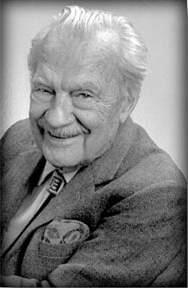
\includegraphics[width=0.9\columnwidth]{nicholas_metropolis.png}
    \end{column}
  \end{columns}
\end{frame}

\begin{frame}{Algoritmo de Metropolis}
  A essência do algoritmo é um passeio aleatório pelo espaço amostral dos parâmetros,
  onde a probabilidade da corrente Markov mudar de estado é definida como:

  $$
  P_{\text{mudar}} = \min\left({\frac{P (\boldsymbol{\theta}_{\text{proposto}})}{P (\boldsymbol{\theta}_{\text{atual}})}},1\right).
  $$

  Isso quer dizer a corrente Markov somente mudará para um novo estado em duas condições:
  \begin{vfilleditems}
    \small
    \item \small Quando a probabilidade dos parâmetros propostos pelo passeio aleatório
    $P(\boldsymbol{\theta}_{\text{proposto}})$ é \textbf{\textcolor{blue}{maior}}
    que a probabilidade dos parâmetros do estado atual
    $P(\boldsymbol{\theta}_{\text{atual}})$, mudamos com 100\% de probabilidade.

    \item \small Quando a probabilidade dos parâmetros propostos pelo passeio aleatório
    $P(\boldsymbol{\theta}_{\text{proposto}})$ é \textbf{\textcolor{red}{menor}}
    que a probabilidade dos parâmetros do estado atual
    $P(\boldsymbol{\theta}_{\text{atual}})$, mudamos com probabilidade igual a
    proporção dessa diferença.
  \end{vfilleditems}
\end{frame}

\begin{frame}[fragile]{Algoritmo de Metropolis}
    \SetAlCapFnt{\normalsize}
    \SetAlCapNameFnt{\normalsize}
    \begin{algorithm}[H]
    \DontPrintSemicolon
    \SetAlgoNoEnd
    \SetAlgoLined
    Defina um ponto inicial $\boldsymbol{\theta}^{(0)} \in \mathbb{R}^p$ do qual $P\left(\boldsymbol{\theta}^{(0)} \mid \boldsymbol{y} \right) > 0$\;
     \Para{$t = 1, 2, \dots$}{
      Amostra uma proposta $\boldsymbol{\theta}^{(*)}$ de uma distribuição de propostas no tempo $t$, $J_t \left(\boldsymbol{\theta}^{(*)} \mid \boldsymbol{\theta}^{(t-1)} \right)$\;
      Como regra de aceitação/rejeição calcule a proporção das probabilidades:
      $r = \frac{P\left(\boldsymbol{\theta}^{(*)}  \mid \boldsymbol{y} \right)}{P\left(\boldsymbol{\theta}^{(t-1)} \mid \boldsymbol{y} \right)}$\;
      Designe:
      $
        \boldsymbol{\theta}^{(t)} =
          \begin{cases}
          \boldsymbol{\theta}^{(*)} & \text{com probabilidade $\min(r,1)$}\\
          \boldsymbol{\theta}^{(t-1)} & \text{caso contrário}
        \end{cases}
      $\;
     }
     \caption{Metropolis}
    \end{algorithm}
\end{frame}

\begin{frame}{Intuição Visual de Metropolis}
\centering
    \begin{tikzpicture}
        \begin{axis}[every axis plot, line width=2pt,
            ylabel=PDF,
            domain=-4:4,samples=200,
            ymax = 0.6, ytick={0, 0.2, 0.4},
            axis x line*=bottom, % no box around the plot, only x and y axis
            axis y line*=left, % the * suppresses the arrow tips
            enlargelimits=true,
            ] % extend the axes a bit

            \addplot [blue] {gaussian(0, 1)};
            \node[inner sep=0pt] (hikerlower) at (-2,0.13){\Strichmaxerl[2pt]};
            \node[inner sep=0pt] (hikerupper) at (0,0.5){\Strichmaxerl[2pt]};
            \node[inner sep=0pt] (hikerlower2) at (2,0.13){\Strichmaxerl[2pt]};
            \draw[->, red, line width=2pt] (hikerlower) to [out=90,in=135] node[above left] {\large$P=1$} (hikerupper);
            \draw[->, yellow, line width=2pt] (hikerupper) to [out=45,in=135] node[right] {\large$P\approx\frac{0.1}{0.4}\approx\frac{1}{4}$} (hikerlower2);
        \end{axis}
        \end{tikzpicture}

\end{frame}

\subsubsection{Metropolis-Hastings}
\begin{frame}{Algoritmo de Metropolis}
  \begin{columns}
    \begin{column}{0.8\textwidth}
      Na década de 1970, surgiu um generalização do algoritmo de Metropolis
      que \textbf{não} necessita que as distribuições de proposta sejam simétricas:
      $$
      J_t (\boldsymbol{\theta}^{(*)} \mid \boldsymbol{\theta}^{(t-1)}) \neq J_t(\boldsymbol{\theta}^{(t-1)} \mid \boldsymbol{\theta}^{(*)})
      $$
      A generalização foi proposta por \href{https://en.wikipedia.org/wiki/W._K._Hastings}{Wilfred Keith Hastings}
      \parencite{hastingsMonteCarloSampling1970} e chama-se algoritmo
      de \textbf{Metropolis-Hastings}.
    \end{column}
    \begin{column}{0.2\textwidth}
      \centering
      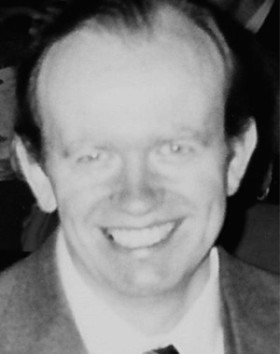
\includegraphics[width=0.9\columnwidth]{hastings.jpg}
    \end{column}
  \end{columns}
\end{frame}

\begin{frame}[fragile]{Algoritmo de Metropolis - Hastings}
    \SetAlCapFnt{\normalsize}
    \SetAlCapNameFnt{\normalsize}
    \small
    \begin{algorithm}[H]
    \DontPrintSemicolon
    \SetAlgoNoEnd
    \SetAlgoLined
    Defina um ponto inicial $\boldsymbol{\theta}^{(0)} \in \mathbb{R}^p$ do qual $P\left(\boldsymbol{\theta}^{(0)} \mid \boldsymbol{y} \right) > 0$\;
     \Para{$t = 1, 2, \dots$}{
      Amostra uma proposta $\boldsymbol{\theta}^{(*)}$ de uma distribuição de propostas no tempo $t$, $J_t \left(\boldsymbol{\theta}^{(*)} \mid \boldsymbol{\theta}^{(t-1)} \right)$\;
      Como regra de aceitação/rejeição calcule a proporção das probabilidades:
      $r = \frac{\frac{P \left(\boldsymbol{\theta}^{(*)} \mid \boldsymbol{y} \right)}{J_t \left(\boldsymbol{\theta}^{(*)} \mid \boldsymbol{\theta}^{(t-1)} \right)}}{\frac{P \left(\boldsymbol{\theta}^{(t-1)} \mid \boldsymbol{y} \right)}{J_t \left(\boldsymbol{\theta}^{(t-1)} \mid \boldsymbol{\theta}^{(*)} \right)}}$\;
      Designe:
      $
        \boldsymbol{\theta}^{(t)} =
          \begin{cases}
          \boldsymbol{\theta}^{(*)} & \text{com probabilidade $\min(r,1)$}\\
          \boldsymbol{\theta}^{(t-1)} & \text{caso contrário}
        \end{cases}
      $\;
     }
     \caption{Metropolis-Hastings}
    \end{algorithm}
\end{frame}

\begin{frame}{Animação Metropolis\footnote{veja Metropolis em ação no \href{https://chi-feng.github.io/mcmc-demo/app.html?algorithm=RandomWalkMH&target=banana}{\texttt{chi-feng/mcmc-demo}}}}
  \centering
  \movie[loop, width=9cm, height=6cm]{Animação Metropolis}{animations/rwmh.m4v}
\end{frame}

\subsubsection{Limitações dos Algoritmos Metropolis}
\begin{frame}{Limitações dos Algoritmos Metropolis}
  As limitações do algoritmo de Metropolis-Hastings são principalmente
  \textbf{computacionais}:
  \begin{vfilleditems}
    \item Com propostas geradas aleatoriamente, geralmente leva um grande número de
    iterações para entrar em áreas de densidade posterior mais alta (mais provável).

    \item Mesmo algoritmos de Metropolis-Hastings eficientes às vezes aceitam menos de
    25\% das propostas \parencite{robertsWeakConvergenceOptimal1997, beskosOptimalTuningHybrid2013}.

    \item Em situações dimensionais mais baixas, o poder computacional aumentado pode compensar a eficiência mais baixa até certo ponto.
    Mas em situações de modelagem de dimensões mais altas e mais complexas, computadores maiores
    e mais rápidos sozinhos raramente são suficientes para superar o desafio.
  \end{vfilleditems}
\end{frame}

\subsubsection{Gibbs}
\begin{frame}{Algoritmo de Gibbs}
  \begin{columns}
    \begin{column}{0.8\textwidth}
      Para contornar o problema de baixa taxa de aceitação dos algoritmos de Metropolis
      foi desenvolvido o algoritmo de Gibbs que
      \textbf{não possui uma regra de aceitação/rejeição}
      para a mudança de estado da corrente Markov:
      \textbf{Todas as propostas são aceitas}!
      \vfill
      O algoritmo de Gibbs teve ideia original concebida pelo físico Josiah Willard Gibbs
      em referência a uma analogia entre um algoritmo de amostragem e a
      física estatística (\textit{statistical physics} um ramo da física que tem sua
      base em mecânica estatística, \textit{statistical mechanics}).
      O algoritmo foi descrito pelos irmãos Stuart e Donald Geman em 1984
      \parencite{gemanStochasticRelaxationGibbs1984}, cerca de oito décadas após
      a morte de Gibbs.
    \end{column}
    \begin{column}{0.2\textwidth}
      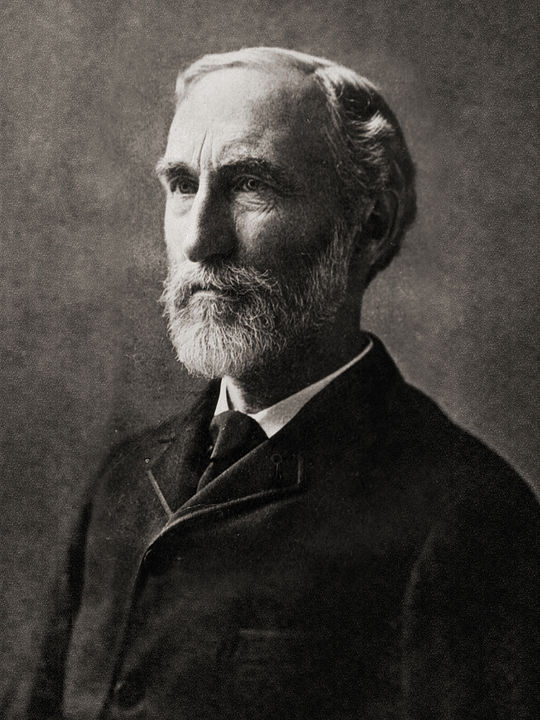
\includegraphics[width=0.9\columnwidth]{josiah_gibbs.jpg}
    \end{column}
  \end{columns}
\end{frame}

\begin{frame}{Algoritmo de Gibbs}
  O algoritmo de Gibbs é muito útil em espaços amostrais multidimensionais\footnote{
  no qual há bem mais que 2 parâmetros a serem amostrados da probabilidade posterior}.
  Também é conhecido como amostragem condicional alternativa
  (\textit{alternating conditional sampling}), pois amostramos sempre um parâmetro
  \textbf{condicionado} à probabilidade dos outros parâmetros do modelo.
  \vfill
  O algoritmo de Gibbs pode ser visto como um \textbf{caso especial} do algoritmo
  de Metropolis-Hastings porque todas as propostas são aceitas
  \parencite{gelmanIterativeNonIterativeSimulation1992}.
  \vfill
  A essência do algoritmo de Gibbs é a amostragem de parâmetros condicionada à outros parâmetros:
  $$P(\theta_1 \mid \theta_2, \dots \theta_p)$$
\end{frame}

\begin{frame}[fragile]{Algoritmo de Gibbs}
    \SetAlCapFnt{\normalsize}
    \SetAlCapNameFnt{\normalsize}
    \begin{algorithm}[H]
    \DontPrintSemicolon
    \SetAlgoNoEnd
    \SetAlgoLined
    Defina um ponto inicial $\boldsymbol{\theta}^{(0)} \in \mathbb{R}^p$ do qual $P\left(\boldsymbol{\theta}^{(0)} \mid \boldsymbol{y} \right) > 0$\;
     \Para{$t = 1, 2, \dots$}{
      Designe:
      $ \boldsymbol{\theta}^{(t)} =
        \begin{cases}
        \theta^{(t)}_1 &\sim P \left(\theta_1 \mid \theta^{(0)}_2, \dots, \theta^{(0)}_p \right) \\
        \theta^{(t)}_2 &\sim P \left(\theta_2 \mid \theta^{(t-1)}_1, \dots, \theta^{(0)}_p \right) \\
        &\vdots \\
        \theta^{(t)}_p &\sim P \left(\theta_p \mid \theta^{(t-1)}_1, \dots, \theta^{(t-1)}_{p-1} \right)
     \end{cases}
      $\;
     }
     \caption{Gibbs}
    \end{algorithm}
\end{frame}

\begin{frame}{Animação Gibbs\footnote{Veja Gibbs em ação no \href{https://chi-feng.github.io/mcmc-demo/app.html?algorithm=GibbsSampling&target=banana}{\texttt{chi-feng/mcmc-demo}}}}
  \centering
  \movie[loop, width=9cm, height=6cm]{Animação Gibbs}{animations/gibbs.m4v}
\end{frame}

\subsubsection{Limitações do Algoritmo de Gibbs}
\begin{frame}{Limitações do Algoritmo de Gibbs}
  A principal limitação do algoritmo de Gibbs é com relação a
  \textbf{amostragem condicional alternativa}:
  \begin{vfilleditems}
    \item Em Metropolis temos propostas aleatórias
    de uma distribuição de propostas na qual amostramos cada parâmetro
    \textbf{incondicionalmente} à outros parâmetros e de maneira \textbf{simultânea} usando a
    probabilidade conjunta desses parâmetros. As mudanças de estado da corrente
    Markov são então executadas \textbf{multidimensionalmente}.
    Isto provoca movimentos "\textbf{diagonais}"~multidimensionais.

    \item No caso do algoritmo de Gibbs essa movimentação se dá apenas em um
    único parâmetro, pois amostramos \textbf{sequencialmente} e
    \textbf{condicionalmente} à outros parâmetros.
    Isto provoca movimentos \textbf{horizontais/verticais} unidimensionais,
    mas nunca movimentos diagonais multidimensionais.
  \end{vfilleditems}
\end{frame}

\subsubsection{Hamiltonian Monte Carlo (HMC)}
\begin{frame}{Classe de Algoritmos MCMC - Hamiltoninan Monte Carlo (HMC)}
  \begin{columns}
    \begin{column}{0.8\textwidth}
      Os problemas de baixas taxas de aceitação de propostas das técnicas de
      Metropolis e do desempenho baixo do algoritmo de Gibbs em problemas
      multidimensionais nas quais a geometria da posterior é complexa
      fizeram com que surgisse uma nova técnica MCMC usando dinâmica Hamiltoniana
      (em homenagem ao físico irlandês
      \href{https://en.wikipedia.org/wiki/William_Rowan_Hamilton}{William Rowan Hamilton}.
    \end{column}
    \begin{column}{0.2\textwidth}
      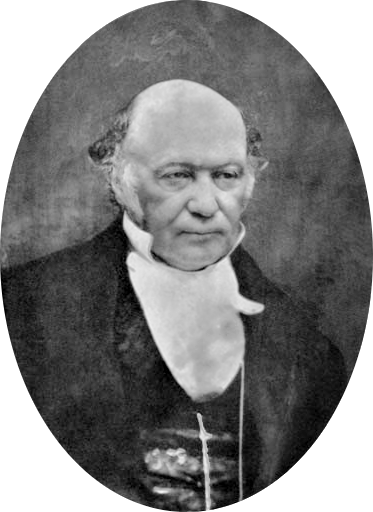
\includegraphics[width=0.9\columnwidth]{hamilton.png}
    \end{column}
  \end{columns}
\end{frame}

\begin{frame}{Algoritmo de HMC}
  O HMC é uma adaptação da técnica de Metropolis e emprega um esquema guiado de
  geração de novas proposta: isso melhora a taxa de aceitação de propostas e,
  consequentemente, a eficiência.
  \vfill
  Mais especificamente, o HMC usa o gradiente do log da posterior para direcionar
  a cadeia de Markov para regiões de maior densidade posterior,
  onde a maioria das amostras são coletadas.
  $$
  \frac{d \log P(\boldsymbol{\theta} \mid \boldsymbol{y})}{d \theta}
  $$
  Como resultado, uma corrente Markov com o algoritmo HMC bem ajustada aceitará
  propostas em uma taxa muito mais alta do que o algoritmo Metropolis tradicional
  \parencite{robertsWeakConvergenceOptimal1997, beskosOptimalTuningHybrid2013}.
\end{frame}

\begin{frame}{História do Algoritmo de HMC}
  HMC foi inicialmente descrito na literatura de física\footnote{que chamaram de \textit{"Hybrid"~Monte Carlo} -- HMC}
  \parencite{duaneHybridMonteCarlo1987}.
  \vfill
  Logo depois, HMC foi aplicado a problemas estatísticos por
  \textcite{nealImprovedAcceptanceProcedure1994} que chamou de \textit{Hamiltonean Monte Carlo}
  -- HMC).
  \vfill
  Para uma discussão aprofundada (que não é o foco deste conteúdo) de HMC eu recomendo
  \textcite{neal2011mcmc} e \textcite{betancourtConceptualIntroductionHamiltonian2017}.
\end{frame}

\begin{frame}{O que muda com HMC?}
  HMC usa dinâmica Hamiltoniana aplicada para partículas explorando de maneira mais
  eficiente a geometria de uma probabilidade posterior.
  \vfill
  Além de explorar melhor a geometria da posterior e tolerar geometrias complexas,
  HMC é muito mais eficiente que Metropolis e não sofre do problema de correlação
  dos parâmetros que Gibbs.
\end{frame}

\begin{frame}{Intuição por trás do Algoritmo de HMC}
  \small
  Para cada componente $\theta_j$, o HMC adiciona uma variável de momento
  $\phi_j$. A densidade posterior $P(\boldsymbol{\theta} \mid y)$ é incrementada
  por uma distribuição independente $P(\boldsymbol{\phi})$ dos momentos,
  definindo assim uma distribuição conjunta:
  $$
  P(\boldsymbol{\theta}, \boldsymbol{\phi} \mid y) = P(\boldsymbol{\phi}) \cdot P(\boldsymbol{\theta} \mid y)
  $$
  \small
  O HMC usa uma distribuição de propostas que muda dependendo do estado atual na
  corrente Markov. O HMC descobre a direção em que a distribuição posterior aumenta,
  chamada de \textit{gradiente}, e distorce a distribuição de propostas em
  direção ao \textit{gradiente}.
  \vfill
  A probabilidade da corrente Markov mudar de estado no algoritmo HMC é definida como:
  $$
  P_{\text{mudar}} = \min\left({\frac{P(\boldsymbol{\theta}_{\text{proposto}}) \cdot P(\boldsymbol{\phi}_{\text{proposto}})}{P(\boldsymbol{\theta}_{\text{atual}})\cdot P(\boldsymbol{\phi}_{\text{atual}})}}, 1\right)
  $$
\end{frame}

\begin{frame}{Distribuição dos Momentos -- $P(\boldsymbol{\phi})$}
  Normalmente damos a $\boldsymbol{\phi}$ uma distribuição normal multivariada
  com média 0 e covariância de $\mathbf{M}$,
  uma "matriz de massa".
  \vfill
  Para mantêr as coisas um pouco mais simples, usamos uma matriz de massa diagonal
  $\mathbf{M}$. Isso faz com que os componentes de $\boldsymbol{\phi}$ sejam
  independentes com
  $$\phi_j \sim \text{Normal}(0, M_{jj})$$
\end{frame}

\begin{frame}[fragile]{Algoritmo de HMC}
    \SetAlCapFnt{\normalsize}
    \SetAlCapNameFnt{\normalsize}
    \begin{algorithm}[H]
    \DontPrintSemicolon
    \SetAlgoNoEnd
    \SetAlgoLined
    \footnotesize
    Defina um ponto inicial $\boldsymbol{\theta}^{(0)} \in \mathbb{R}^p$ do qual $P\left(\boldsymbol{\theta}^{(0)} \mid \boldsymbol{y} \right) > 0$\;
    Amostre $\boldsymbol{\phi}$ de uma $\text{Normal}(\mathbf{0},\mathbf{M})$\;
    Simultaneamente amostre $\boldsymbol{\theta}^{(*)}$ e $\boldsymbol{\phi}$ com $L$ passos e tamanho de passo $\epsilon$.\;
    Defina o valor atual $\boldsymbol{\theta}$ como valor proposto $\boldsymbol{\theta}^{(*)}$:
    $\boldsymbol{\theta}^{(*)} \leftarrow \boldsymbol{\theta}$\;
    \Para{$1, 2, \dots, L$}{
     Use o gradiente do $\log$ da posterior de $\boldsymbol{\theta}^{(*)}$ para produzir um meio-passo de $\boldsymbol{\phi}$:
     $\boldsymbol{\phi} \leftarrow \boldsymbol{\phi} + \frac{1}{2} \epsilon \frac{d \log P(\boldsymbol{\theta}^{(*)} \mid \boldsymbol{y})}{d \theta}$\;
     Use $\boldsymbol{\phi}$ para atualizar $\boldsymbol{\theta}^{(*)}$:
     $\boldsymbol{\theta}^{(*)} \leftarrow \boldsymbol{\theta}^{(*)} + \epsilon \mathbf{M}^{-1} \boldsymbol{\phi}$\;
     Novamente use o gradiente de $\boldsymbol{\theta}$ para produzir um meio-passo de $\boldsymbol{\phi}$:
     $\boldsymbol{\phi} \leftarrow \boldsymbol{\phi} + \frac{1}{2} \epsilon \frac{d \log P(\boldsymbol{\theta}^{(*)} \mid \boldsymbol{y})}{d \theta}$\;
    }
    Como regra de aceitação/rejeição calcule:
    $r = \frac{P \left(\boldsymbol{\theta}^{(*)} \mid \boldsymbol{y} \right) P \left(\boldsymbol{\phi}^{(*)} \right)}{P \left(\boldsymbol{\theta}^{(t-1)} \mid \boldsymbol{y} \right) P \left(\boldsymbol{\phi}^{(t-1)} \right)}$\;
    Designe:
      $
        \boldsymbol{\theta}^{(t)} =
          \begin{cases}
          \boldsymbol{\theta}^{(*)} & \text{com probabilidade $\min(r,1)$}\\
          \boldsymbol{\theta}^{(t-1)} & \text{caso contrário}
        \end{cases}
      $\;
    \caption{Hamiltonian Monte Carlo (HMC)}
    \end{algorithm}
\end{frame}

\begin{frame}{Animação HMC\footnote{Veja HMC em ação no \href{https://chi-feng.github.io/mcmc-demo/app.html?algorithm=HamiltonianHMC&target=banana}{\texttt{chi-feng/mcmc-demo}}}}
  \centering
  \movie[loop, width=9cm, height=6cm]{Animação HMC}{animations/hmc.m4v}
\end{frame}

\begin{frame}{Um interlúdio de Integrador Numéricos}
  No campo das equações diferenciais ordinais temos a ideia de discretizar um
  sistema de equações diferenciais ordinais ao aplicar um pequeno passo $\epsilon$\footnote{algumas vezes também chamado de $h$}.
  Tais abordagem são chamadas de \textbf{integradores numéricos} e comportam uma
  \textbf{ampla classe} de ferramentas.
  \vfill
  O mais famoso e simples desses integradores numéricos é o método de Euler. No qual
  usa-se um tamamho de passo $\epsilon$ para calcular a solução numérica do estado
  em um futuro tempo $t$ a partir de condições iniciais específicas.
\end{frame}

\begin{frame}{Um interlúdio de Integrador Numéricos}
  \begin{columns}
    \begin{column}{0.6\textwidth}
      O problema é que o método de Euler quando aplicado para dinâmicas Hamiltonianas
      é que ele não preserva o volume. Uma das propriedades fundamentais das dinâmicas
      Hamiltonianas é que elas preservam volume, um resultado chamado de Teorema de
      Liouville. Isto faz com que o método de Euler seja uma péssima escolha como
      integrador numérico de um algoritmo HMC.
    \end{column}
    \begin{column}{0.4\textwidth}
      \begin{figure}
      \includegraphics[width=0.8\columnwidth]{euler_0_3.jpg}
      \caption{Método de Euler num algoritmo HMC com $\epsilon = 0.3$ e $L = 20$}
      \end{figure}
    \end{column}
  \end{columns}
\end{frame}

\begin{frame}{Um interlúdio de Integrador Numéricos\footnote{Um excelente livro-texto
  para integradores numéricos e integradores simpléticos é
  \textcite{irseles2008numericalanalysis}}}
  \begin{columns}
    \begin{column}{0.6\textwidth}
      Para preservação de volumes precisamos usar um
      \textbf{integrador simplético}. Integradores simpléticos são no máximo
      de ordem 2 e precisam ser usados com um tamanho de passo $\epsilon$ constante.
      Um dos principais integradores numéricos simpléticos usado em dinânimcas
      Hamiltonianas é o integrador \textbf{Störmer–Verlet}, também conhecido
      como \textit{leapfrog}.
    \end{column}
    \begin{column}{0.4\textwidth}
      \begin{figure}
        \includegraphics[width=0.8\columnwidth]{leapfrog_0_3.jpg}
        \caption{Integrador \textit{Leapfrog} num algoritmo HMC com $\epsilon = 0.3$ e $L = 20$}
        \end{figure}
    \end{column}
  \end{columns}
\end{frame}

\begin{frame}{Limitações do Algorito HMC}
  \begin{columns}
    \begin{column}{0.6\textwidth}
      Como vocês podem ver o algoritmo de HMC é muito sensível a escolhe da quantidade
      de passos $L$ e do tamanho do passo $\epsilon$. Em especial o integrador
      \textit{leapfrog} permite apenas um $\epsilon$ constante, portanto temos um
      equilíbrio delicado entre $L$ e $\epsilon$. Em  termos algorítmicos, $L$
      e $\epsilon$ são hiperparâmetros (tem que ser cuidadosamente ajustados).
    \end{column}
    \begin{column}{0.4\textwidth}
      \begin{figure}
        \includegraphics[width=0.8\columnwidth]{leapfrog_1_2.jpg}
        \caption{Integrador \textit{Leapfrog} num algoritmo HMC com $\epsilon = 1.2$ e $L = 20$}
        \end{figure}
    \end{column}
    \end{columns}
\end{frame}

\subsubsection{No-U-Turn-Sampler (NUTS)}
\begin{frame}{\textbf{N}o-\textbf{U}-\textbf{T}urn-\textbf{S}ampler (NUTS)}
  Em HMC, conseguimos ajustar o $\epsilon$ durante a execução do algoritmo. Mas, geralmente
  precisamos executar algumas vezes o amostrador HMC para ajustar o $L$.
  \vfill
  Aqui vem a ideia do \textbf{N}o-\textbf{U}-\textbf{T}urn-\textbf{S}ampler (NUTS)
  \parencite{hoffman2014no}.
  Não é preciso ajustar \textbf{nada} apenas "apertar"~o botão. Ele calcula automaticamente
  $\epsilon$ e $L$.
\end{frame}

\begin{frame}{\textbf{N}o-\textbf{U}-\textbf{T}urn-\textbf{S}ampler (NUTS)}
  Mais especificamente precisamos de um critério que informe que já simulamos as dinâmicas
  Hamiltonianas por "tempo suficiente". \textit{i.e.} simular as dinâmicas por mais tempo
  não aumentaria a distância entre a proposta $\boldsymbol{\theta}^{(*)}$ e o valor atual
  $\boldsymbol{\theta}$.
  \vfill
  NUTS então usa um critério baseado no produto interno entre os vetores do momento
  atual $\boldsymbol{\phi}$ e a diferença entre os vetores
  da proposta $\boldsymbol{\theta}^{(*)}$ e o valor atual $\boldsymbol{\theta}$,
  que é a derivada com respeito ao tempo $t$ de metade da distância ao quadrado
  entre $\boldsymbol{\theta}$ e $\boldsymbol{\theta}^{(*)}$
  $$
  (\boldsymbol{\theta}^{(*)} - \boldsymbol{\theta}) \cdot \boldsymbol{\phi}
  = (\boldsymbol{\theta}^{(*)} - \boldsymbol{\theta}) \cdot \frac{d}{dt} (\boldsymbol{\theta}^{(*)} - \boldsymbol{\theta})
  = \frac{d}{dt} \frac{(\boldsymbol{\theta}^{(*)} - \boldsymbol{\theta}) \cdot (\boldsymbol{\theta}^{(*)} - \boldsymbol{\theta})}{2}
  $$
\end{frame}

\begin{frame}{\textbf{N}o-\textbf{U}-\textbf{T}urn-\textbf{S}ampler (NUTS)}
  Isso sugere um algorimo que não permite com que as propostas sejam guiadas de maneira
  infinita até que a distância entre a proposta $\boldsymbol{\theta}^{(*)}$ e o valor atual
  $\boldsymbol{\theta}$ seja menor que zero.
  \vfill
  Isto quer dizer que tal algoritmo não \textbf{permitirá meia-voltas} (\textit{u-turns}).
\end{frame}

\begin{frame}{\textbf{N}o-\textbf{U}-\textbf{T}urn-\textbf{S}ampler (NUTS)}
  NUTS usa o integrador \textit{leapfrog} para criar uma árvore binária da qual os nós-folha
  são as posições do momento $\boldsymbol{\phi}$ traçando tanto um caminho para frente
  ($t+1$) quanto para trás ($t-1$) em um tempo fictício em um determinado tempo $t$.
  O crescimento dos nós-folha são \textbf{interrompidos} quando é detectado meia-volta
  tanto para frente quanto para trás.
  \begin{figure}
    \centering
    \includegraphics[width=0.6\textwidth]{nuts.jpg}
    \caption{NUTS crescendo nós-folha para frente}
  \end{figure}
\end{frame}

\begin{frame}{\textbf{N}o-\textbf{U}-\textbf{T}urn-\textbf{S}ampler (NUTS)}
  NUTS também um procedimento chamado \textit{Dual Averaging}
  \parencite{nesterov2009primal} para ajustar simultaneamente $\epsilon$ e $L$ ao
  considerar o produto $\epsilon \cdot L$.
  \vfill
  Tal ajuste é feito durante a fase de \textit{warmup} e os valores definidos de
  $\epsilon$ e $L$ são mantidos fixos durante a fase de amostragem.
\end{frame}

\begin{frame}{Algoritmo de NUTS}
    \SetAlCapFnt{\footnotesize}
    \SetAlCapNameFnt{\footnotesize}
    \begin{algorithm}[H]
    \DontPrintSemicolon
    \SetAlgoNoEnd
    \SetAlgoLined
    \fontsize{4.5pt}{6.5pt}\selectfont
    Defina um ponto inicial $\boldsymbol{\theta}^{(0)} \in \mathbb{R}^p$ do qual $P\left(\boldsymbol{\theta}^{(0)} \mid \boldsymbol{y} \right) > 0$\;
    \textcolor{blue}{Inicie uma árvore binária vazia com $2^L$ nós}\;
    Amostre $\boldsymbol{\phi}$ de uma $\text{Normal}(\mathbf{0},\mathbf{M})$\;
    Simultaneamente amostre $\boldsymbol{\theta}$ e $\boldsymbol{\phi}$ com $L$ passos e tamanho de passo $\epsilon$.\;
    Defina o valor atual $\boldsymbol{\theta}$ como valor proposto $\boldsymbol{\theta}^{(*)}$:
    $\boldsymbol{\theta}^{(*)} \leftarrow \boldsymbol{\theta}$\;
    \Para{$1, 2, \dots, 2L$}{
     \textcolor{blue}{Escolha uma direção $v \sim \text{Uniforme}\left( \left\{-1, 1 \right\} \right)$}\;
     Use o gradiente do $\log$ da posterior de $\boldsymbol{\theta}^{(*)}$ para produzir um meio-passo de $\boldsymbol{\phi}$ na direção $v$:
     $\boldsymbol{\phi} \leftarrow \boldsymbol{\phi} + v \frac{1}{2} \epsilon \frac{d \log P(\boldsymbol{\theta}^{(*)} \mid \boldsymbol{y})}{d \theta}$\;
     Use $\boldsymbol{\phi}$ para atualizar $\boldsymbol{\theta}^{(*)}$:
     $\boldsymbol{\theta}^{(*)} \leftarrow \boldsymbol{\theta}^{(*)} + \epsilon \mathbf{M}^{-1} \boldsymbol{\phi}$\;
     Novamente use o gradiente de $\boldsymbol{\theta}^{(*)}$ para produzir um meio-passo de $\boldsymbol{\phi}$ na direção $v$:
     $\boldsymbol{\phi} \leftarrow \boldsymbol{\phi} + v \frac{1}{2} \epsilon \frac{d \log P(\boldsymbol{\theta}^{(*)} \mid \boldsymbol{y})}{d \theta}$\;
     Defina o nó $L_t^v$ como a proposta $\boldsymbol{\theta}$\;
     \eSe{
       A diferença entre os vetores
       da proposta $\boldsymbol{\theta}^{(*)}$ e o valor atual $\boldsymbol{\theta}$ na direção $v$ for menor que zero: $v \frac{d}{dt} \frac{(\boldsymbol{\theta}^{(*)} - \boldsymbol{\theta}^{(*)}) \cdot (\boldsymbol{\theta}^{(*)} - \boldsymbol{\theta}^{(*)})}{2} < 0$\;
     }{
       \textcolor{red}{Pare a amostragem de $\boldsymbol{\theta}^{(*)}$ na direção $v$ e continue apenas amostrando na direção $-v$}\;
       }{
        \Se{A distância entre os vetores
        da proposta $\boldsymbol{\theta}^{(*)}$ e o valor atual $\boldsymbol{\theta}$ na direção restante $-v$ for menor que zero: $-v \frac{d}{dt} \frac{(\boldsymbol{\theta}^{(*)} - \boldsymbol{\theta}^{(*)}) \cdot (\boldsymbol{\theta}^{(*)} - \boldsymbol{\theta}^{(*)})}{2} < 0$\;
       }{
        \textcolor{red}{Pare a amostragem de $\boldsymbol{\theta}^{(*)}$\;
        }
       }
     }
    }
    Como regra de aceitação/rejeição calcule:
    $r = \frac{P \left(\boldsymbol{\theta}^{(*)} \mid \boldsymbol{y} \right) P \left(\boldsymbol{\phi}^{(*)} \right)}{P \left(\boldsymbol{\theta}^{(t-1)} \mid \boldsymbol{y} \right) P \left(\boldsymbol{\phi}^{(t-1)} \right)}$\;
    Designe:
      $
        \boldsymbol{\theta}^{(t)} =
          \begin{cases}
          \boldsymbol{\theta}^{(*)} & \text{com probabilidade $\min(r,1)$}\\
          \boldsymbol{\theta}^{(t-1)} & \text{caso contrário}
        \end{cases}
      $\;
    \caption{No-U-Turn-Sampler (NUTS)}
    \end{algorithm}
\end{frame}

\begin{frame}{Animação NUTS\footnote{Veja NUTS em ação no \href{https://chi-feng.github.io/mcmc-demo/app.html?algorithm=EfficientNUTS&target=banana}{\texttt{chi-feng/mcmc-demo}}}}
  \centering
  \movie[loop, width=9cm, height=6cm]{Animação NUTS}{animations/nuts.m4v}
\end{frame}

\subsubsection{Limitações de HMC e NUTS}
\begin{frame}{Limitações do Algorito HMC e NUTS - Funil de \textcite{nealSliceSampling2003}}
  O famoso funil da morte \footnote{muito comum em modelos hierárquicos}.
  Aqui vemos que os algoritmos HMC e NUTS, durante a exploração da
  posterior, tem que a todo momento trocar valores\footnote{lembre-se que
  $\epsilon$ e $L$ são definidos na fase de \textit{warmup} e
  mantidos fixos durante a fase de amostragem} de $\epsilon$ e $L$.
% https://crackedbassoon.com/writing/funneling
% import numpy as np
% import matplotlib
% import matplotlib.pyplot as plt
% from matplotlib import rcParams
% from scipy.stats import norm
% fs = rcParams["figure.figsize"]
% rcParams["figure.figsize"] = (fs[0], fs[0] / 2)
% rcParams["lines.linewidth"] = 2
% rcParams["font.size"] = 14
% rcParams["axes.edgecolor"] = 'b'
% rcParams["xtick.labelcolor"] = 'w'
% rcParams["ytick.labelcolor"] = 'w'


% # generate data
% np.random.seed(0)
% k = 9
% n = 10000
% v = norm.rvs(0, 3, n)
% x = norm.rvs(0, np.exp(v / 2), (k, n))

% # plot data and analytic log-likelihood
% r = 500
% x, v = np.meshgrid(np.linspace(-20, 20, r), np.linspace(-9, 9, r))
% logp = norm.logpdf(v, 0, 3) + norm.logpdf(x, 0, np.exp(v / 2))
% plt.imshow(logp, vmin=-7.5, vmax=-2.5, cmap="viridis", origin="lower")
% plt.xticks(np.linspace(0, 499, 5), labels=np.linspace(-20, 20, 5).astype(int))
% plt.yticks(np.linspace(0, 499, 5), labels=np.linspace(-9, 9, 5).astype(int))

% # save figure
% plt.savefig('slides/images/funnel.png', bbox_inches=0, transparent=True, dpi=300)
  \centering
  \includegraphics[width=0.65\textwidth]{funnel.png}
\end{frame}

\begin{frame}{Funil de \textcite{nealSliceSampling2003} e Parametrização Não-Centralizada\footnote{\textit{Non-Centered Parametrization} (NCP)}}
  \small
  O funil ocorre quando temos uma variável que a sua variância depende da variância
  de outra em uma escala exponencial. Um exemplo canônico de uma parametrização
  centralizada é:
  $$
  P(y,x) = \text{Normal}(y \mid 0 ,3) \cdot
  \text{Normal}\left(x \mid 0, e^{\left(\frac{y}{2}\right)}\right)
  $$
  Isto ocorre bastante em modelos hierárquicos, na relação dos \textit{prioris} de grupo
  com a(s) \textit{hiperpriori(s)} global(is). Então, reparametrizamos de maneira
  não-centrada alterando a geometria da posterior para facilitar a vida do amostrador
  MCMC:
  $$
  \begin{aligned}
    P(\tilde{y},\tilde{x}) &= \text{Normal}(\tilde{y} \mid 0, 1) \cdot
  \text{Normal}(\tilde{x} \mid 0, 1) \\
    y &= \tilde{y} \cdot 3 + 0 \\
    x &= \tilde{x} \cdot  e^{\left(\frac{y}{2}\right)} + 0
  \end{aligned}
  $$
\end{frame}

\begin{frame}{\href{https://mc-stan.org}{\texttt{Stan}} e NUTS}
  \href{https://mc-stan.org}{\texttt{Stan}} foi o primeiro amostrador MCMC a
  implementar NUTS. Além disso tem uma rotina otimizada automática de ajuste de $L$
  e $\epsilon$ durante a fase de \textit{warmup}. Possui os seguintes valores como
  hiperparâmetros padrões do NUTS\footnote{para mais informações sobre como
  modificar esses hiperparâmetros consulte a \href{
    https://mc-stan.org/docs/reference-manual/hmc-algorithm-parameters.html}{
    Seção 15.2 do \textit{Stan Reference Manual}}}:
  \begin{vfilleditems}
    \item \textbf{Taxa-alvo de aceitação de propostas Metropolis}: \lstinline!adapt_delta = 0.8!
    \item \textbf{Profundidade máxima de árvore} (em potências de 2): \lstinline!max_treedepth = 10! (quer dizer $2^{10} = 1024$)
  \end{vfilleditems}
\end{frame}

\subsection{Convergência de Correntes Markov}
\begin{frame}{Convergência de Correntes Markov}
  MCMC tem uma propriedade interessante que é garantido que \textbf{assintoticamente ele convergirá
  à distribuição-alvo}.
  \vfill
  Ou seja, se tivermos todo o tempo do mundo, é garantido que, irrelevante da geometria
  da distribuição-alvo (posterior), \textbf{MCMC irá lhe dar a resposta correta}.
  \vfill
  Porém não temos todo o tempo do mundo. Diferentes algoritmos MCMC, como HMC e NUTS,
  podem reduzir o tempo de amostragem (e \textit{warmup}) necessários para convergência.
\end{frame}

\subsubsection{Métricas de Convergência}
\begin{frame}{Métricas de Convergência}
  Temos algumas maneiras de mensurar se as correntes Markov convergiram à distribuição-alvo,
  \textit{i.e.} são "confiáveis":
  \begin{vfilleditems}
    \item Número de Amostras Efetivas (\textit{Effective Sample Size} -- ESS):
    uma aproximação do "número de amostras independentes"~geradas por uma corrente Markov.
    \item $\widehat{R}$ (\textit{Rhat}):
    escala de \textbf{R}edução potencial, uma métrica de mensuração que as correntes
    Markov se "misturaram", e, potencialmente, convergiram
  \end{vfilleditems}
\end{frame}

\begin{frame}{Métricas de Convergência - \textit{Effective Sample Size} \parencite{gelman2013bayesian}}
  $$\widehat{n}_{\text{eff}} = \frac{mn}{1 + \sum_{t=1}^T \widehat{\rho}_t}$$
  Onde:
  \begin{vfilleditems}
    \item $m$: número de correntes Markov
    \item $n$: amostras totais por corrente Markov (descontando \textit{warmup})
    \item $\widehat{\rho}_t$: uma estimativa de autocorrelação
  \end{vfilleditems}
\end{frame}

\begin{frame}{Métricas de Convergência - \textit{Rhat} \parencite{gelman2013bayesian}}
  $$\widehat{R} = \sqrt{\frac{\widehat{\text{var}}^+(\psi \mid y)}{W}}$$
  onde a $\widehat{\text{var}}^+(\psi \mid y)$ é a variância das amostras das
  correntes Markov para um determinado parâmetro $\psi$ sob uma média ponderada
  das variâncias intra-correntes (\textit{within-chain}) $W$ e inter-correntes
  (\textit{between-chain}) $B$
  $$\widehat{\text{var}}^+(\psi \mid y) = \frac{n-1}{n} W + \frac{1}{n} B$$
  Intuitivamente, seu valor é $1.0$ se as correntes estiverem totalmente convergentes.
  Como uma heurística, se $\widehat{R}$ for maior que $1.1$, você deve se preocupar pois
  provavelmente as correntes não tenham convergido adequadamente.
\end{frame}

\subsubsection{Visualizações de Convergência}
\begin{frame}{\textit{Traceplot} -- Correntes Markov Convergentes}
  \begin{figure}
    \centering
    \resizebox{.4\linewidth}{!}{\input{images/good_chains_traceplot.tex}}
  \end{figure}
\end{frame}

\subsubsection{O que fazer se Correntes Markov não Convergirem}

\begin{frame}[fragile]{\textit{Rhat} -- Mensagens de Erro do \href{https://mc-stan.org}{\texttt{Stan}}\footnote{além disso não deixe de checar o \href{https://mc-stan.org/misc/warnings.html}{guia dos \textcolor{red}{\textit{warnings}} do \texttt{Stan}}}}
  \begin{lstlisting}[basicstyle=\footnotesize\color{red}]
Warning messages:
1: There were 275 divergent transitions after warmup. See
http://mc-stan.org/misc/warnings.html#divergent-transitions-after-warmup
to find out why this is a problem and how to eliminate them.
2: Examine the pairs() plot to diagnose sampling problems

3: The largest R-hat is 1.12, indicating chains have not mixed.
Running the chains for more iterations may help. See
http://mc-stan.org/misc/warnings.html#r-hat
4: Bulk Effective Samples Size (ESS) is too low, indicating posterior
means and medians may be unreliable.
Running the chains for more iterations may help. See
http://mc-stan.org/misc/warnings.html#bulk-ess
5: Tail Effective Samples Size (ESS) is too low, indicating posterior
variances and tail quantiles may be unreliable.
Running the chains for more iterations may help. See
http://mc-stan.org/misc/warnings.html#tail-ess
  \end{lstlisting}
\end{frame}
% https://mc-stan.org/misc/warnings.html

\begin{frame}{\textit{Traceplot} -- Correntes Markov Divergentes}
  \begin{figure}
    \centering
    \resizebox{.4\linewidth}{!}{\input{images/bad_chains_traceplot.tex}}
  \end{figure}
\end{frame}

\begin{frame}{O que fazer se Correntes Markov não Convergirem}
  \textbf{Primeiro}: Antes de fazer ajustes finos no número de correntes
  \texttt{chains} ou no número de iterações \texttt{iter} (entre outros ...)
  saiba que o amostrador HMC-NUTS do \href{https://mc-stan.org}{\texttt{Stan}} e
  seu ecossistema de pacotes (\href{http://mc-stan.org/rstanarm/}{\texttt{rstanarm}} e
  \href{https://paul-buerkner.github.io/brms/}{\texttt{brms}} inclusos) é \textbf{muito
  eficiente e eficaz em explorar as mais diversas complexas e "malucas"~geometrias}
  de distribuições-alvo posterior.
  \vfill
  Os argumentos padrões, \texttt{iter = 2000}, \texttt{chains = 4} e
  \texttt{warmup = floor(iter / 2)}, funcionam perfeitamente para 99\% dos casos
  (mesmo em modelos complexos).
\end{frame}

\begin{frame}{O que fazer se Correntes Markov não Convergirem}
  \vfill
  Dito isto, \textbf{na maioria das vezes quando você
  possui problemas de amostragem e computacionais no seu modelo Bayesiano, o problema
  está na especificação do modelo e não no algoritmo de amostragem MCMC}\footnote{Esta
  frase foi dita por Andrew Gelman (o "pai"~do \texttt{Stan}) e é conhecido como o
  \textit{Folk Theorem} \parencite{gelmanFolkTheoremStatistical2008}:
  \textit{"When you have computational problems, often there’s a problem with
  your model"}}
\end{frame}

\begin{frame}{O que fazer se Correntes Markov não Convergirem}
  Se o seu modelo Bayesiano está com problemas de convergência há alguns
  passos que podem ser tentados\footnote{além disso,
  vale a pena ativar a decomposição QR na matriz $\mathbf{X}$ de dados, criando uma
  base ortogonal (não correlacionada) para amostragem. Isso faz com a distribuição-alvo
  (posterior) fique muito mais amigável do ponto de vista topológico/geométrico
  para o amostrador MCMC explorá-la de maneira mais eficiente e eficaz.}.
  Aqui listados do mais simples para o mais complexo:
  \begin{vfilleditems}
    \item \textbf{Aumentar o número de iterações e correntes}: primeira opção
    é aumentar o número de iterações do MCMC com o argumento \texttt{iter = XXX}
    e também é possível aumentar o número de correntes com o argumento
    \texttt{chains = X}. Lembrando que o padrão é \texttt{iter = 2000} e
    \texttt{chains = 4}.
  \end{vfilleditems}
\end{frame}

\begin{frame}{O que fazer se Correntes Markov não Convergirem}
  \begin{vfilleditems}
    \item \textbf{Alterar a rotina de adaptação do HMC}: a segunda opção é fazer com
    que o algoritmo de amostragem HMC fique mais conservador
    (com proposições de pulos menores). Isto pode ser alterado com o argumento
    \texttt{adapt\_delta} da lista de opções \texttt{control}.
    \texttt{control = list(adapt\_delta = 0.9)}. O padrão do \texttt{adapt\_delta} é $0.8$.
    Então qualquer valor entre $0.8$ e $1.0$ o torna mais conservador.
    \item \textbf{Reparametrização do Modelo}: a terceira opção é reparametrizar o
    modelo. Há duas maneiras de parametrizar o modelo: a primeira com parametrização
    centrada (\textit{centered parameterization}) e a segunda com parametrização
    não-centrada (\textit{non-centered parameterization}).
  \end{vfilleditems}
\end{frame}

\begin{frame}{O que fazer se Correntes Markov não Convergirem}
  \begin{vfilleditems}
    \item \textbf{Coletar mais dados}: às vezes o modelo é complexo demais e
    precisamos de uma amostragem maior para conseguirmos estimativas estáveis.
    \item \textbf{Repensar o modelo}: falha de convergência quando temos uma
    amostragem adequada geralmente é por conta de uma especificação de \textit{prioris} e
    verossimilhança que não são compatíveis com os dados. Nesse caso, é preciso
    repensar o processo generativo de dados no qual os pressupostos do modelo
    estão ancorados.
  \end{vfilleditems}
\end{frame}
